%%%%%%%%%%%%%%%%%%%%%%%%%%%%%%%%%%%%%%%%%%%%%%%%%%%%%%%%%%%%%%%%%%%%%%%%%%%%
%% Trim Size: 9.75in x 6.5in
%% Text Area: 8in (include Runningheads) x 5in
%% ws-ijfcs.tex: 05-05-2015
%% Tex file to use with ws-ijfcs.cls written in Latex2E.
%% The content, structure, format and layout of this style file is the
%% property of World Scientific Publishing Co. Pte. Ltd.
%% Copyright 2015 by World Scientific Publishing Co.
%% All rights are reserved.
%%%%%%%%%%%%%%%%%%%%%%%%%%%%%%%%%%%%%%%%%%%%%%%%%%%%%%%%%%%%%%%%%%%%%%%%%%%%
%

\documentclass{ws-ijfcs}
\usepackage{enumerate}
\usepackage{textcomp}
\usepackage{url}
\usepackage{graphicx}
\usepackage[numbers]{natbib}
\usepackage{bussproofs}
\usepackage{tikz}
\usepackage{amssymb}
\usepackage{amsmath}
\usepackage[all,cmtip]{xy}
\usetikzlibrary{positioning, automata}
\usetikzlibrary{decorations.pathmorphing}
 \usetikzlibrary{snakes}


\tikzset{snake it/.style={decorate, decoration=snake}}
\urlstyle{same}
\begin{document}

\markboth{E. Shemetova, A. Okhotin, S. Grigorev}
{The Parallel Complexity of CFL-Reachability Problem:
Tractable Cases
}

%%%%%%%%%%%%%%%%%%%%% Publisher's Area please ignore %%%%%%%%%%%%%%%
%
\catchline{}{}{}{}{}
%
%%%%%%%%%%%%%%%%%%%%%%%%%%%%%%%%%%%%%%%%%%%%%%%%%%%%%%%%%%%%%%%%%%%%

\title{The Parallel Complexity of CFL-Reachability Problem:
Tractable Cases\footnote{
This research was supported by the Russian Science Foundation, grant \textnumero 18-11-00100.}}
%using \LaTeX\footnote{For the title, try not to use more than 3
%lines. Typeset the title in 10 pt Roman, boldface with the first letter of
%important words capitalized.}}%

\author{Ekaterina Shemetova\footnote{
St. Petersburg State University, 
7/9 Universitetskaya nab., Saint Petersburg 199034, Russia.}
\footnote{
St. Petersburg Academic University, 
ul. Khlopina, 8, Saint Petersburg 194021, Russia.}
\footnote{
JetBrains Research,
Primorskiy prospekt 68-70, Building 1, St. Petersburg, 197374, Russia.}
}

\address{
\email{katyacyfra@gmail.com}}

\author{Alexander Okhotin\footnotemark[2] }

\address{
\email{alexander.okhotin@spbu.ru}
}

\author{Semyon Grigorev\footnotemark[2] \footnotemark[4] }

\address{
\email{s.v.grigoriev@spbu.ru}
}


\maketitle

\begin{history}
\received{(Day Month Year)}
%\revised{(Day Month Year)}
\accepted{(Day Month Year)}
%\comby{(xxxxxxxxxx)}
\end{history}

\begin{abstract}
Whereas it has been shown that  context-free language (CFL) reachability problem is P-complete, there are some subclasses of context-free languages, for which CFL-reachability lies in NC complexity class. We present two common classes which generalize known examples of such tractable subclasses: bounded-oscillation languages and context-free languages with a poly-slender storage languages. Polynomiality of the rational indices of languages in these classes is proved. Also closure properties of tractable subclasses in terms of polynomial rational index are investigated.
\end{abstract}

\keywords{CFL-reachability; parallel complexity; digraphs; regular languages; context-free languages; context-free path queries.}

\section{Introduction}
\label{intro}
The context-free language (CFL) reachability problem for a context-free grammar $G$ and directed edge-labeled graph $D$ consists of determining for pairs of nodes  $v$ and $u$ whether $v$ can reach $u$ via a path labeled by a string in $L(G)$.  That is, CFL-reachability is a kind of graph reachability problem with path constraints given by context-free languages. It is an important problem underlying some fundamental static code analysis like data flow analysis and program slicing \cite{RepsBasic}, alias analysis \cite*{Chatterjee, alias}, points-to analysis \cite{Incremental} and other \cite{Cai, android, typeflow}, and graph database query evaluation \cite{Azimov, GrigorevRagozina, HellingsCFPQ, RDF}.


Unlike context-free language recognition, which is in NC (when context-free grammar is fixed), CFL-reachability is P-complete \cite{ RepSeq, Yannakakis}. Practically, it means that there is no efficient parallel algorithm for solving this problem (unless P $\neq$ NC). 


While problem is not parallelizable in general, it is useful to develop more efficient parallel solutions for specific subclasses of context-free languages. For example, there are context-free languages which admit more efficient parallel algorithms in comparison with the general case of context-free recognition \cite{IBARRA, IBARRA2, Okhotin2014ComplexityOI}.  The same holds for CFL-reachability problem: there are some examples of context-free languages, for which CFL-reachability problem lies in NL complexity class (for example, linear and one-counter languages) \cite{labelledGraphs, LReach, Regularrealizability}. 


CFL-reachability problem has long been known to be P-complete \cite{PCompl}. A parallel complexity of this problem is studied by both static code analysis \cite{RepSeq, RepsBasic} and database communities \cite{ChainQ, Ullman, Yannakakis}. First investigations of such type were made in terms of Datalog queries, because some classes of Datalog queries (chain queries) can be represented via context-free grammars, while database can be considered as a graph. 
\begin{example}[Datalog chain query as a context-free grammar]
Consider the following Datalog query which determines all pairs of people $x$ and $y$ such that a person $x$ is a descendant of a person $y$: 


$Desc(x, y)$ :- $Child(x, y)$

$Desc(x, y)$ :- $Child(x, z), Desc(z, y)$


This query can be represented as a context-free grammar with the following rules: 


$Desc \rightarrow Child$ $\vert$ $Child$ $Desc$


$Child  \rightarrow child$


Thus, evaluating the above mentioned Datalog query is equivalent to the solving the CFL-reachability problem for a context-free grammar representation of this query and an edge-labeled graph representing database, where every person is represented by a node and edges are labeled with a word ``$child$''. 
\end{example}
Important decidability result is obtained in \cite{Vardi}: given a context-free grammar (query) and an arbitrary graph (database), it is undecidable whether CFL-reachability problem for them is in NC or P-complete. However, Ulman and Van Gelder in \cite{Ullman} introduce a notion of a  \textit{polynomial fringe property} and show that the CFL-reachability problem for context-free grammars having this property and an arbitrary graph is in NC. A context-free grammar $G$ has the \textit{polynomial fringe property} if and only if there is a polynomial $p$ such that, for each regular language $R$ recognized by an automaton with $n$ states, $L(G) \cap R$ is either empty or contains a word shorter than $p(n)$. It is undecidable whether a context-free grammar has the polynomial fringe property. Important results from \cite{Ullman} can be reinterpreted in terms of CFL-reachability as follows: 
\begin{enumerate}
\item CFL-reachability for linear languages and piecewise linear languages, and for arbitrary graphs is in NC, because corresponding grammars have the polynomial fringe property
\item The same holds for $D_1$ (the Dyck language on one kind of parentheses) and its GSM-mappings (one-counter languages)
\item CFL-reachability for $D_2$ (the Dyck language on two kinds of parentheses) is P-complete.
\end{enumerate}
The third result is important because any context-free language can be represented via a regular language and $D_2$, which are combined by means of an intersection and a homomorphism, so it is the direct consequence of P-completeness of CLF-reachability problem in general. Also, using the fact that $D_2$ is included in many interesting subclasses of context-free languages, such as visibly pushdown languages \cite{Okhotin2014ComplexityOI}, simple deterministic languages (defined by LL(1) grammars in Greibach normal form), we can state that CFL-reachability for these languages is P-complete. Afrati et al. \cite{ChainQ} investigate parallel complexity of Datalog simple chain queries and presents the Polynomial Stack Lemma which will be discussed in detail in Section~\ref{sec:poly}. 


The definition of polynomial fringe property coincides with the notion of a so called \textit{rational index}: for a context-free language $L(G)$ having the polynomial rational index is the same as for $G$ to have the polynomial fringe property. More precisely, rational index $\rho_L(n)$ is a function, which denotes the maximum length of the shortest word in $L(G) \cap R$, for arbitrary $R$ recognized by an $n$-state automaton. The notion of rational index was introduced in \cite{RatBasic} as a complexity measure for context-free languages and was investigated independently from the polynomial fringe property.  In particular, it has been proved that the rational index of $D_1$ is in $O( n^2)$ \cite{Dyck1}. 
Another important result concerns the rational index of languages, which generate all context-free languages (an example of such language is $D_2$). It states that the rational index of such languages is of the order $exp(\Theta(n^2/\ln n))$ \cite{CFRat} and, hence, this is the upper bound on the value of rational index for every context-free language. An example of a non-generating language with exponential rational index is given in \cite{Regularrealizability}. Also it has been shown that for every algebraic number $\gamma $ the language with the rational index in $\Theta (n^\gamma )$ exists \cite{GreibRat}. 


The CFL-reachability problem is the same as the intersection non-emptiness problem for a context-free language (pushdown automaton) and a regular language (finite automaton), because a labeled graph is a special kind of a nondeterministic finite automaton. Complexity of this problem is studied by Ganardi et al. \cite{ ganardi2016circuit} ,  Swernofsky et al. \cite{Intersection}, Vyalyi \cite{VyalyiRR}.


Computational complexity of the language reachability for different variants of languages (regular, context-free, context-sensitive) and graphs (acyclic graphs, trees, grid graphs) is discussed in detail by Barret et al. \cite{Barrett}, Holzer et al.\cite{labelledGraphs}, Komarath et al. \cite{LReach}. 


\begin{figure}
\centering
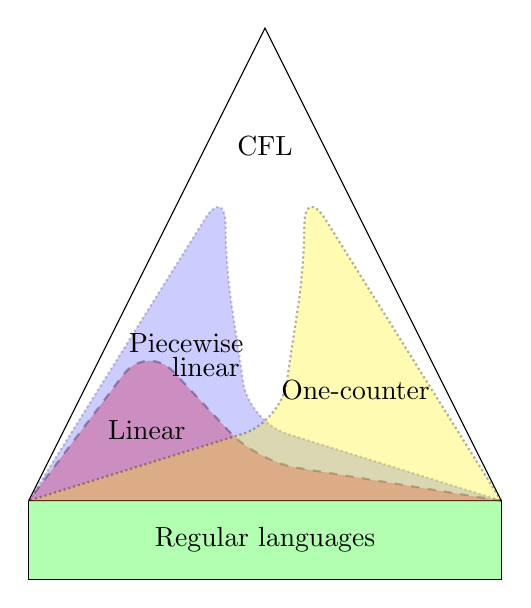
\begin{tikzpicture}
\draw[fill=green, opacity=0.3](0,1) -- (0,0) -- (6,0) --  (6,1);
\draw(0,1) -- (0,0) -- (6,0) --  (6,1);
\draw(0,1) -- (6,1) -- (3, 7) -- (0,1) ;
%\draw[thick, dashed, rounded corners=5mm, fill=yellow, opacity=0.3] (0,1) -- (3.1, 1.5) -- (4.5, 3) -- (6,1);
\draw[thick, dashed, rounded corners=5mm, fill=red, opacity=0.3] (6,1) -- (2.9, 1.5) -- (1.5, 3) -- (0,1);
\draw[thick, densely dotted, rounded corners=5mm, fill=blue, opacity=0.2](0,1) -- (2.5, 5) -- (2.5,4)-- (2.8, 2) -- (6,1);
\draw[thick, densely dotted, rounded corners=5mm , fill=yellow, opacity=0.3](6,1) -- (3.5, 5) -- (3.5,4)-- (3.2, 2) -- (0,1);
\node (reg) at (3, 0.5) {Regular languages}; 
\node (cfl) at (3, 5.5) {CFL}; 
\node (lin) at (1.5, 1.9) {Linear}; 
\node (one) at (4.15, 2.4) {One-counter}; 
\node (linsc) at (2, 3) {Piecewise};
\node (linpsc) at (2.25, 2.7)  {linear}; 
\end{tikzpicture}
\caption{The hierarchy of languages, for which CFL-reachability problem is in NC.}
\label{hierarchy}      
\end{figure}
Our focus is on investigating the parallel complexity of CFL-reachability. Especially we are interested in generalization of ``easy'' subclasses and discovering new examples of context-free languages, for which CFL-reachability is in NC. Effective subclasses can be useful in practice, because the general problem is not tractable \cite{ExperimentalCFPQ}. For example, in case of graph databases it is important to know the complexity of a given context-free path query. Also it is natural to ask which properties of subclasses imply parallel effectiveness. Why some languages have polynomial rational indices? What is the difference between them and other subclasses of context-free languages?


The hierarchy of subfamilies of context-free languages, for which the CFL-reachability problem is in NC, is presented in Figure~\ref{hierarchy}. Linear (and piecewise linear) languages and one-counter languages are incomparable families of context-free languages, but both have polynomial rational indices (polynomial fringe property). These subfamilies have one thing in common: both are defined by strong restrictions on the stack in a pushdown automaton. Our main idea is to generalize known tractable classes by investigating the restrictions on the PDA store.

\textbf{Our contributions.} Our results can be summarized as follows:
\begin{itemize}
\item We show that the CFL-reachability problem for bounded-oscillation languages of Ganty and Valput \cite{BoundOsc}, is in NC (see Section \ref{sec:osc}). This class generalizes the case of linear languages. 
\item Closure properties of the languages with polynomial rational indices are investigated in Section \ref{sec:closure}, particularly it is shown that the family of languages with polynomial rational is closed under Kleene star and insertion of a regular language.
\item In Section \ref{sec:poly} we introduce a new subclass of context-free languages --- context-free languages with a poly-slender pushdown store languages. These languages are the natural generalization of one-counter languages, and the CFL-reachability problem for them is in NC. Also we show that deciding poly-slenderness of a pushdown store language is in P.
\end{itemize}


\section{Preliminaries}

In this section we introduce common definitions in graph theory and formal language theory which will be used in this paper. 
Also, we provide brief description of Azimov's algorithm which is used as a base of our solution.

\subsection{Graphs}

In this work we use edge-labelled digraph as a data model and define it as follows.
\begin{definition} \emph{Labeled directed graph} is a triple $D = (V,E,\sigma)$, where
\begin{itemize}
    \item $V$ is a set of vertices
    \item $E$ is a set of edges
    \item $\sigma \subseteq \Sigma$ is a set of labels, and a set of edges $E\subseteq V\times \sigma \times V$
\end{itemize}
\end{definition}

An example of the graph is presented in figure~\ref{fig:example_input_graph}.

\begin{figure}[h]
    \centering        
    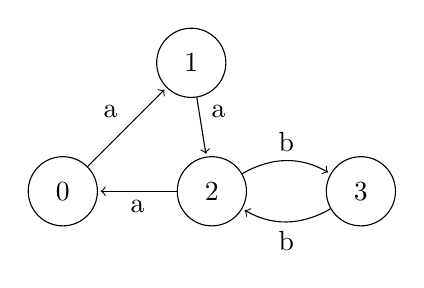
\begin{tikzpicture}[shorten >=1pt,auto]
       \node[state] (q_0)                      {$0$};
       \node[state] (q_1) [above right=of q_0] {$1$};
       \node[state] (q_2) [right=of q_0]       {$2$};
       \node[state] (q_3) [right=of q_2]       {$3$};
        \path[->]
        (q_0) edge  node {a} (q_1)
        (q_1) edge  node {a} (q_2)
        (q_2) edge  node {a} (q_0)
        (q_2) edge[bend left, above]  node {b} (q_3)
        (q_3) edge[bend left, below]  node {b} (q_2);
    \end{tikzpicture}
    \caption{The example of input graph $\mathcal{G}$}
    \label{fig:example_input_graph}
\end{figure}

We use adjacency matrix decomposed to a set of a boolean matrix as a representation of the graph.
\begin{definition}
An adjacency matrix $M$ of the graph $\mathcal{G}=$ is a square $|V|\times|V|$ matrix, such that $M[i,j] = \{l \mid e = (i,l,j) \in E\}$.
\end{definition}

Adjacency matrix $M$ of the graph $\mathcal{G}$ is

$$
    M =
    \begin{pmatrix}
    . & \{a\} & . & .     \\
    . & . & \{a\} & .     \\
    \{a\} & . & . & \{b\} \\
    . & . & \{b\} & .
    \end{pmatrix}.
$$

\begin{definition}

Boolean decomposition of adjacency matrix $M$ of graph $\mathcal{G}=$ is set of Boolean matrix $$\mathcal{M} = \{M^l \mid l \in L, M^l[i,j]=1 \iff l \in M[i,j]\}.$$

\end{definition}

Matrix $M$ can be represented as a set of two Boolean matrices $M^a$ and $M^b$ where
\begin{align}
M^{a} =
\begin{pmatrix}
    . & 1 & . & .   \\
    . & . & 1 & .   \\
    1 & . & . & .   \\
    . & . & . & .  
\end{pmatrix}, 
M^{b} =
\begin{pmatrix}      
    . & . & . & .   \\
    . & . & . & .   \\
    . & . & . & 1   \\
    . & . & 1 & . 
\end{pmatrix} \label{eq:boolean_decomposition_of_graph}
\end{align}
\subsection{Languages}

\begin{definition}\emph{Context-free grammar} is a 4-tuple $G=(N, \Sigma, R, S)$, where 
\begin{itemize}
    \item $N$ is a set of nonterminals
    \item $\Sigma$ is a set of terminals
    \item $R$ is a finite set of productions of the followings form: $A \to \alpha, ~A \in N,~ \alpha \in (N \cup \Sigma)^*$
    \item $S$ - a starting nonterminal
\end{itemize}
\end{definition}

\begin{definition} \emph{Context-free language} is a language generated by a context-free grammar:
\begin{align*}
     L(G) = \{w \in \Sigma^* \mid S \Rightarrow^* w \} 
\end{align*}
Where $S \Rightarrow^* w$  denotes that a string $w$ can be generated from a starting non-terminal $S$ using some sequence of production rules from $P$.
\end{definition}

\begin{definition} Context-free grammar $G = (N, \Sigma, R, S)$ is said to be in \emph{Chomsky normal form} if all productions in $R$ are of the form:
    \begin{itemize}
        \item $A \rightarrow BC,~A,~B,~C \in N$
        \item  $A \rightarrow a,~A \in N,~a \in \Sigma$
        \item $S \rightarrow \varepsilon,~\varepsilon$ is an empty string
    \end{itemize}
\end{definition}
Note that every context-free grammar can be transformed into an equivalent one in Chomsky Normal Form. 
\begin{definition} Context-free grammar $G = (N, \Sigma, P, S)$ is said to be in \emph{Weak Chomsky normal form} if all productions in $P$ are of the form:
    \begin{itemize}
        \item $A \rightarrow BC,~A,~B,~C \in N$
        \item  $A \rightarrow a,~A \in N,~a \in \Sigma$
        \item $A \rightarrow \varepsilon,~A \in N$
    \end{itemize}
\end{definition}
In other words, weak Chomsky normal form differs from Chomsky normal Form in the followings:
\begin{itemize}
    \item $\varepsilon$ can be derived from any non-terminal
    \item $S$ can be at a right part of productions
\end{itemize}
    
    
For example, let's consider the following context-free grammar, which generates the language $L(G) = \{A^nB^n, n \in \mathbb{N}\}$:
$G=(N, \Sigma, P, S), ~N=\{S\},~\Sigma=\{A,B\}$ and productions: 
\begin{align*}
S \rightarrow AB \\
S \rightarrow ASB\\
S \rightarrow \varepsilon
\end{align*}
After transformation to Chomsky Normal Form the resulting grammar:
\begin{align*}
S \rightarrow AB \\
S \rightarrow AC \\
C \rightarrow SB \\
S \rightarrow \varepsilon
\end{align*}

This productions itself are the grammar that has the same result as original grammar.

We use a context-free grammar in the weak Chomsky Normal Form without a starting non-terminal, which will be specified in the path queries for the graph. It should be noted that we omit the rules of the form $A \rightarrow \varepsilon$ for the reason that they correspond to trivial paths, which are more convenient to consider separately.

\begin{definition}\emph{Context-free relation} is a relation $R_A \subseteq V \times V$ for graph $G = (V, E)$, context-free grammar $G = (N,~\Sigma,~P)$ and fixed non-terminal $A$:
\begin{align*}
     R_A = \{(n, m) \mid \exists n \pi m~(l(\pi) \in L(G_A))\}
\end{align*}
\end{definition}

 Now, the definition for \emph{multiple-source (single-source) context-free path querying problem} can be formulated in the introduced notation as follows. For the given graph $G = (V, E)$, context-free grammar $G=(N, \Sigma, P)$ and set of source vertices $Src$ we need to find all context-free relations $R_A$ for any $A \in Src$. 
 
\subsection{Matrix-Based Algorithm}
Let $D = (V, E)$ be the input graph and $G = (N, \Sigma, P)$ be the input grammar. For the context-free path query evaluation, we need to provide context-free relations \mbox{$R_A \subseteq V \times V$} for every \mbox{$A \in N$}.
The matrix-based algorithm for CFPQ can be expressed in terms of operations over Boolean matrices (see listing~\ref{alg:algo0}) which is an advantage for implementation.
{\footnotesize
\begin{algorithm}
\begin{algorithmic}[1]
\caption{Context-free path querying algorithm}
\label{alg:algo0}
\Function{evalCFPQ}{$D=(V,E), G=(N,\Sigma,P)$}
    \State{$n \gets$ |V|}
    \State{$T \gets \{T^{A_i} \mid A_i \in N, T^{A_i}$ is a matrix $n \times n$, $T^{A_i}_{k,l} \gets$ \texttt{false}\} }
    \ForAll{$(i,x,j) \in E$, $A_k \mid A_k \to x \in P$}
        %\Comment{Matrices initialization}
        %\For{$A_k \mid A_k \to x \in P$}
          {$T^{A_k}_{i,j} \gets \texttt{true}$}
        %\EndFor
    \EndFor
    \ForAll{$A_k \mid A_k \to \varepsilon \in P$}
        \ForAll{$i \in \{0,\ldots ,n-1\}$}
            {$T^{A_k}_{i,i} \gets \texttt{true}$}
        \EndFor
    \EndFor

    \While{any matrix in $T$ is changing}
        %\Comment{Transitive c	losure calculation}
        \For{$A_i \to A_j A_k \in P$}
          { $T^{A_i} \gets T^{A_i} + (T^{A_j} \times T^{A_k})$ } 
        \EndFor
    \EndWhile
\State \Return $T$
\EndFunction
\end{algorithmic}
\end{algorithm}
}

This CFPQ algorithm allows efficiently apply GPGPU techniques, but it solves all-pairs problem and takes unreasonable amount of memory in scenarios in which we want to find paths from a relatively small set of vertices, since it calculates a lot of redundant information.  
\section{Rational index of bounded-oscillation languages}
\label{sec:osc}
\subsection{Upper bounds on the rational index of bounded oscillation languages}
Before we consider the value of the rational index for $k$-bounded-oscillation languages, we need to prove the following.
\begin{lemma}
\label{lem:treeheight}
Let  $G = (\Sigma, N, P, S)$ be a context-free grammar in Chomsky normal form,  $D=(V, E, \Sigma)$ be a directed labeled graph with $n$ nodes. Let $w$ be the shortest string in $L(G)\cap L(D)$. Then the height of every parse tree for $w$ in $G$ does not exceed $|N|n^2$.
\end{lemma}

\begin{proof}
Consider grammar $G'$ for $L(G)\cap L(D)$. The grammar $G = (\Sigma, N', P', S')$ can be constructed from $G$ using the classical Bar-Hillel et al. \cite{BarHillel} construction: $N' \subseteq N \times V \times V $  contains all tiples $(A, i, j)$ such that $A \in N, i, j \in V$ ; $P'$ contains production rules in one of the following forms:
\begin{enumerate}
\item $(A, i, j) \rightarrow (B, i, k), (C, k, j)$ for all $(i, k, j)$ in $V$  if $A \rightarrow BC \in P$
\item $(A, i, j) \rightarrow a$ for all $(i, j)$ in $V$ if $A \rightarrow a$.
\end{enumerate}
A triple $(A, i, j)$ is \textit{realizable} iff there is a path $i\pi j$ such that $A \stackrel {*}{\Rightarrow } l(\pi)$ for some nontermimal $A \in N$. Then the parse tree $t_G$ for $w$ in $G$ can be converted into parse tree $t_{G'}$ in $G'$. Notice that every node of $t_{G'}$ is realizable triple. Also it is easy to see that the height of $t_G$ is equal to the height of $t_{G'}$. Assume that $t_{G'}$ for $w$ has a height of more than $|N|n^2$. Consider a path from the root of the parse tree to a leaf, which has length greater than $|N|n^2$. There are $|N|n^2$ unique labels $(A, i, j)$ for nodes of the parse tree, so according to the pigeonhole principle, this path has at least two nodes with the same label. This means that the parse tree for $w$ contains at least one subtree $t$ with label $(A, i, j)$ at the root, which has a subtree $t'$ with the same label. Then we can change $t$ with $t'$ and get a new string $w'$ which is shorter than $w$, because the grammar is in Chomsky normal form. But $w$ is the shortest, then we have a contradiction.

\end{proof}
From Lemma \ref{lem:treeheight} one can deduce an alternative proof of the fact that the rational index of linear languages is in $O(n^2)$ \cite{RatBasic}: the number of leaves in a parse tree in linear grammar in Chomsky normal form is proportional to its height, and thus it is in $O(n^2)$.
\begin{lemma}
\label{oscbnddim}
Let $G$ be a grammar $G = (\Sigma, N, P, S)$ in Chomsky normal form, such that every parse tree $t$ has $dim(t) \le d$, where $d$ is some constant. Let $D=(V, E, \Sigma)$ be a directed labeled graph with $n$ nodes. Then $\rho_{L(G)}$ is in $O(h^d)$ in the worst case.
\end{lemma}
\begin{proof}
Proof by induction on dimension $dim(t)$.
\\
\textbf{Basis.} $dim(t) = 1$.
\\
Consider a tree $t$ with the dimension $dim(t) = 1$. The root of the tree has the same dimension and has two children (because the grammar is in Chomsky normal form). There are two cases:  first, when both of child nodes have dimension equal to 0, then the tree has only two leaves, and second, when one of the children has dimension 1, and the second child has dimension 0. For the second case we can recursively construct a tree with the maximum number of leaves in the following way. Every internal node of such a tree has two children, one of which has dimension equal to 0 and therefore has only one leaf. This means that the number of leaves (and, hence, $\rho_{L(G)}$) in such a tree is bounded by its height and is in $O(h)$. 
\\
\textbf{Inductive step.} $dim(t) = d + 1$.
\\
Assume that $\rho_{L(G)}$ is at most $O(h^{d})$ for every $d$ in the worst case, where $h$ is the height of the tree. We have two cases for the root node with dimension equal to $d+1$: 1) both of children have a dimension equal to $d$, then by proposition the tree of heght $h$ has no more than $O(h^{d})$ leaves; 2) one of the children has a dimension $d + 1$, and the second child $v$ has a dimension $dim(v) \le d$. Again, a tree with the maximum number of leaves can be constructed recursively:  each node of such tree has two children $u$ and $v$ with dimensions $d+1$ and $d$ respectively (the greater the dimension of the node, the more leaves are in the corresponding tree in the worst case). By the induction assumption there are no more than $(h-1)^d + (h-2)^d + (h-3)^d + ... + 1 = O(h^{d+1})$ leaves, so the claim holds for $dim = d+1$.
\end{proof}
Combining Lemma \ref{lem:treeheight} and Lemma \ref{oscbnddim}, we can deduce the following.
\begin{corollary}
\label{finaldim}
Let $G$ be a grammar $G = (\Sigma, N, P, S)$ in Chomsky normal form, such that every parse tree $t$ has $dim(t) \le d$, where $d$ is some constant. Let $D=(V, E, \Sigma)$ be a directed labeled graph with $n$ nodes. Then $\rho_{L(G)}$ is in $O({(|N|n^2)}^d)$ in the worst case.
\end{corollary}
\begin{theorem}
\label{oscbndosc}
Let $L$ be a $k$-bounded-oscillation language with grammar $G = (\Sigma, N, P, S)$ in Chomsky normal form and $D=(V, E, \Sigma)$ be a directed labeled graph with $n$ nodes. Then $\rho_{L(G)}$ is in $O({|N|}^{2k}n^{4k})$ in the worst case.
\end{theorem}
\begin{proof}
By Lemma~\ref{boscdim}, every parse tree of bounded-oscillation language has also bounded dimension. Then the maximum value of the dimension of every parse tree of $k$-bounded-oscillation language is $2k$. By Corrolary~\ref{finaldim}, $\rho_{L(G)}$ is in $O({(|N|n^2)}^d)$ and, thus, $\rho_{L(G)}$ does not exceed $O({(|N|n^2)}^{2k}) = O({|N|}^{2k}n^{4k})$.
\end{proof}

As we can see from the proof of Lemma~\ref{oscbnddim}, the family of linear languages is included in the family of bounded-oscillation languages. The reason is that the family of bounded-oscillation languages generalizes the family of languages accepted by finite-turn pushdown automata \cite{BoundOsc}. It is interesting that for general PDA, particularly for $D_2$, the value of osciillation is not constant-bounded: it depends on the length of input and does not exeed $O(\log n)$ for the input of length $n$ \cite*{Gundermann, Wechsung}. However, for some previously studied subclasses of context-free languages,  oscillation is bounded by a constant.

\begin{subsection}{The rational indices of some subclasses of bounded-oscillation languages.} 

\paragraph{Superlinear languages.} 
A context-free grammar $G = (\Sigma, N, P, S)$ is \textit{superlinear} \cite{superlinear} if all productions of $P$ satisfy these conditions:
\begin{enumerate}
\item there is a subset $N_L \subseteq N$ such that every $A \in N_L$ has only linear productions $A\rightarrow aB$ or $A\rightarrow Ba$, where $B \in N_L$ and $a \in \Sigma$.
\item if $A \in N \setminus N_L$, then $A$ can have non-linear productions of the form $A \rightarrow BC$ where $B\in N_L$ and $C \in N$, or linear productions of the form $A\rightarrow \alpha B$ $\vert$ $B \alpha$ $\vert$ $\alpha$ for $B \in N_L$, $\alpha \in \Sigma^*$.
\end{enumerate}
A language is \textit{superlinear} if it is generated by some superlinear grammar. 
\begin{theorem} Let $G$ be a superlinear grammar. Then $\rho_{L(G)}$ is in $O(n^4)$.
\end{theorem}
\begin{proof}
From the definition of superlinear grammar $G$ it is observable that its parse trees have dimension at most 2. From 
Corrolary~\ref{finaldim}, if dimensions of all parse trees are bounded by some $k$ then the rational index $\rho_{L(G)}$ of such language is in $O(n^4)$.
\end{proof}
\end{subsection}
\paragraph{Ultralinear languages.} A context-free grammar $G = (\Sigma, N, P, S)$ is \textit{ultrealinear} if there exists a partition $\{N_0, N_1, ..., N_k\}$ of $N$ such that $S \in N_k$ and if $A \in N_i$, where $0 \le i \le k$, then $(A \rightarrow w) \in P$ implies $w \in \Sigma^*N_i\Sigma^*$ or $w \in {(\Sigma \cup N_0 \cup ... \cup N_i-1)}^*$. Such a partition is called an \textit{ultralinear decomposition}. A language is \textit{ultralinear} if it is generated by some ultralinear grammar. 


The ultralinear languages were originally defined by Ginsburg and Spanier \cite{Ginsburg1966FiniteTurnPA} as languages recognizable by finite-turn pushdown PDAs (a finite-turn PDA is a PDA with a fixed constant bound on the number of switches between push and pop operations in accepting computation paths). 

Every ultralinear language is generated by an ultralinear grammar in \textit{reduced form} \cite{WORKMAN1976188}.
\begin{definition}[The reduced form of ultralinear grammar.]
An ultralinear grammar $G = (\Sigma, N, P, S)$ is in \textit{reduced form} if its ultralinear decomposition $\{N_0, N_1, ..., N_k\}$ is in the following form:
\begin{enumerate}
\item $N_k=\{S\}$ and $S$ does not appear in the right part of any production rule
\item if $(A \rightarrow w) \in P \setminus \{S \rightarrow \varepsilon\}$ and $A \in N_i$, $0 \le i \le k$, then $w \in (\Sigma \cup N_i\Sigma \cup \Sigma N_i \cup N_jN_j')$, where $j, j' < i$.
\end{enumerate}
\end{definition}
\begin {theorem}
Let $G = (\Sigma, N, P, S)$ be an ultralinear grammar with the ultralinear decomposition $\{N_0, N_1, ..., N_k\}$. Then $\rho_{L(G)}$ is in $O(n^{2k})$.
\end{theorem}
\begin{proof}
Recall that by definition dimension of a parse tree is the height of its largest perfect subtree. Consider the maximum possible size of a perfect subtree which occurs in the parse tree in ultralinear grammar in reduced form. It is easy to see that the rules of the form $A \rightarrow BC$, where $A \in N_i, B, C \in N_{i-1}$ should be used as often as possible to construct the largest binary subtree. Therefore, if grammar has the subset of rules of the form $\{S \rightarrow AB, A \rightarrow A_1A_2, B \rightarrow B_1B_2, A_1\rightarrow A_3A_4, ..., A_i \rightarrow A_{i+2}, A_{i+3}, ...\}$, where $A, B \in N_{k-1}, A_1, A_2, B_1, B_2 \in N_{k-2}, A_3, A_4, ... \in N_{k-3}, ... , A_{i+2}, A_{i+3}, ... \in N_0$, the perfect binary subtree obtained with these rules will be of height not greater than $k$, so the maximum dimension of the parse tree in a ultralinear grammar in reduced form is $k$. By Corrolary~\ref{finaldim}  $\rho_{L(G)}$ is in $O(n^{2k})$.
\end{proof}
\section{Closure properties of languages with polynomial rational indices}
\label{sec:closure}
Given a context-free language $L$ with the polynomial rational index, it is interesting to find which language operations preserve this property.  Boasson et al. \cite{RatBasic} give the following useful relations for polynomial indices of two languages $L$ and $L'$.
\begin{lemma}[\cite{RatBasic}]
\label{lem:closure}
Context-free languages with polynomial rational indices are closed under intersection with a regular language, union, concatenation, the Kleene star, homomorphism and inverse homomorphism. More precisely,
\begin{itemize}
\item $\rho_{L \cup L'}(n) \le  \max{(\rho_L(n), \rho_{L'}(n))} $
\item $\rho_{LL'}(n) \le \rho_L(n) + \rho_{L'}(n)$
\item $\rho_{L^{*}}(n) \le n(\rho_L(n))$
\item $\rho_{L \cap R}(n) \le \rho_L(nm)$, where $R$ is a regular language recognised by an $m$-state automaton
\item $\rho_{h(L)}(n) \le \rho_L(n)$ and $\rho_{h^{-1}(L)}(n) < n(\rho_L(n) +1)$, where $h: \Sigma^* \rightarrow \Delta^*$ is a homomorphism
\item $\rho_{\tau(L)}(n) \le (mn + 1)\rho_L(mn)$, where $\tau$ is a rational transduction and $m$ is some integer.
\end{itemize}
\end{lemma}
 From the relations above it is easy to see that the family of context-free languages with polynomial rational indices is a full trio. Every full trio is closed under left and right quotient with regular languages, prefix, suffix, infix, and outfix \cite{GinsburgAlgebraic}. Obviously, CFLs with the polynomial rational indices languages are closed under reversal.  Next we show that context-free languages with the polynomial rational indices are closed under insertion of a regular language.
\begin{theorem}
Context-free languages with the polynomial rational indices are closed under the insertion of a regular language. 
\\Particularly, $\rho_{L_{INSERT(K)}}(n) \le (mn + 1)\rho_L(mn)$, where $m$ is the number of states in the NFA accepting $K$.
\end{theorem}
\begin{proof}
 Let $L$ be a language with the polynomial rational index over an alphabet $\Sigma$ and $K$ be a regular language over an alphabet $\Delta$, where an NFA $M(K)$ with $m$ states is an NFA accepting $K$.  Define a homomorphism $h: \Delta^*  \rightarrow \bar{\Delta}^{*}$, such that $h(a)=\bar{a}$,  $\forall a \in \Delta$. In simple words, $h$ makes all symbols from $\Delta$ ``marked''. Then, by defining a homomorphism $g$, such that $g(a) = \varepsilon$, $\forall a \in \bar{\Delta}$ ($g$ erases the symbols of $\bar{\Delta}$), one can insert an arbitrary number of symbols from $\bar{\Delta}$ into strings in $L$ using an inverse homomorphism $g^{-1}$. To obtain a string from $L_{INSERT(K)}$ it is left to intersect $g^{-1}(L)$ with a regular set $K'$ containing strings in the form $xyz$, where $x, z \subseteq \Sigma^{*}$ and $y \in h(K)$. Then ``marked'' symbols from  $\bar{\Delta}$ is unmarked by a homomorphism $\phi:  \bar{\Delta^*}  \rightarrow \Delta^{*}$, where $\phi(\bar{a}) = a$, $\forall \bar{a} \in \bar{\Delta}$. Finally, every word $w' \in L_{INSERT(K)}$ can be written as $\phi(g^{-1}(w) \cap K') = \tau(w)$, where $w \in L$ and $\tau$ is a rational transduction. By Lemma~\ref{lem:closure}, languages with the polynomial rational indices are closed under rational trunsductions, so $L_{INSERT(K)}$ has the polynomial rational index. An NFA $M(K')$ can be easily constructed from $M(K)$ and has $O(m)$ states. Then the value of the rational index $\rho_{L_{INSERT(K)}}(n) \le (mn + 1)\rho_L(mn)$.
\end{proof}



Using closure properties, it is easier to find new subclasses of context-free languages for which the CFL-reachability problem is in NC.
\begin{example}[Metalinear languages \cite{metalinear}.]
Let $G = (\Sigma, N, P, S)$ be a context-free grammar. $G$ is \textit{metalinear} if all productions of $P$ are of the following forms:
\begin{enumerate}
\item $S \rightarrow A_1A_2...A_k$, where $A_i \in N \setminus \{S\}$
\item $A \rightarrow u$, where $A \in N \setminus \{S\}$ and $u \in (\Sigma^*((N \setminus \{S\}) \cup {\varepsilon})\Sigma^*)$
\end{enumerate}


The width of a metalinear grammar is $max\{k\vert S \rightarrow A_1A_2...A_k \}$. Metalinear languages of width 1 are obviously linear languages. It is easy to see that every metalinear language is a union of concatenations of $k$ linear languages. Linear languages have polynomial rational index,  CFLs with the polynomial rational index are closed under concatenation and union, so metalinear languages have the polynomial rational index and, hence, is in NC.
\end{example}


\section{Languages with poly-slender store languages}
\label{sec:poly}
In the previous section restriction of PDA in terms of variability of stack height was described. But this is not the case for $D_1$, which is not $k$-oscillating CFL for any $k$, but has the polynomial rational index. In this section another kind of stack restriction is considered --- poly-slenderness of a pushdown store language as a measure of how stack contents vary along accepting computations of PDA.


For a PDA $M$, its \textit{pushdown store language} $P(M)$ consists of all words
occurring on the stack along accepting computations of $M$. It is well-known that the store language of any PDA is regular. The language $D_1$ is a one-counter language, so its pushdown store language is $Z^*Z_0$, where $Z$ is a single pushdown symbol and $Z_0$ is a bottom symbol $Z_0$.


Afrati et al. \cite{ChainQ} define the notion of \textit{polynomial stack property} and show that if a PDA has the polynomial stack property, then corresponding query has the polynomial fringe property (and hence, lies in NC). A PDA has the polynomial stack property iff the largest possible number of different contents of the same height $k$ along the any accepting computation of $M$ is bounded by polynomial $O(k^d)$ for $d \ge 0$.  For example, the usual PDA for $D_1$ has the polynomial stack property, because there is only one possible variant of contents for every stack height. 


Generalizing an example of the family of one-counter languages, we can define the family of languages whose PDAs have the polynomial stack property --- languages with a \textit{poly-slender} pushdown store language (or storage language with polynomial density). The density of a language is a function $f(n)$ that shows the number of words of length $n$ in language. A language $L \subseteq \Sigma^*$ is called \textit{poly-slender language (or with the polynomial density)} if the function $f(n)$ is bounded by $O(n^k)$ for some $k \ge 0$. For example, the language $Z^*Z_0$ is of polynomial density (even of a constant density), whereas the language ${(Z_1 + Z_2)}^*Z_0$ is of exponential density.


The property of having a poly-slender storage language implies the polynomial stack property, but the converse is not true: there are PDAs with a storage language of an exponential density, which have the polynomial stack property. Consider the language of even-length palindromes $L = \{ ww^R \ | w \in {\{0, 1\}}^*\}$. It is easy to see that usual PDA $M$ for this language has the storage language $P(M) = {(0 + 1)}^*$, which is of an exponential density. But the language $L$ is linear and  the PDA $M$ is a finite-turn automaton, therefore $M$ has bounded stack heights during every accepting computation, and, hence, has the polynomial stack property. 


Whereas the polynomial fringe property of a query is undecidable \cite{Ullman}, it is decidable in polynomial time whether a given PDA has a poly-slender storage language. At first, for a given NFA it is decidable whether its language has a polynomial or exponential density \cite*{sparseness, poldens}. Gawrychowski et al. \cite{Gawrychowski} give an algorithm for testing whether $L(M)$ is of polynomial or exponential density in $O(|Q| + |\delta|)$ time for an NFA $M = (Q,\Sigma,\delta ,q_{0},F)$. An NFA for pushdown store language of a given PDA $\mathcal{A} = (Q', \Sigma', \Gamma, \delta', q_0', Z_0, F')$ can be constructed directly in $O({|Q'|}^5{|\Gamma|}^2|\delta'|)$ time \cite{Malcher}. This construction uses the notion of meaningful triples, which form the states of NFA. A triple $[p, Z, q] \in Q' \times \Gamma \times Q'$ is \textit{meaningful} if there exists a computation of $\mathcal{A}$ starting from state $p$ with the sole symbol $Z$ in the pushdown, and ending in $q$ with the empty pushdown. By definition, there are at most $|\Gamma|{|Q'|}^2$ meaningful triples, and, hence, states of NFA. 



\section{Conclusions and open problems}
\label{sec:conc}
\begin{figure}
\centering
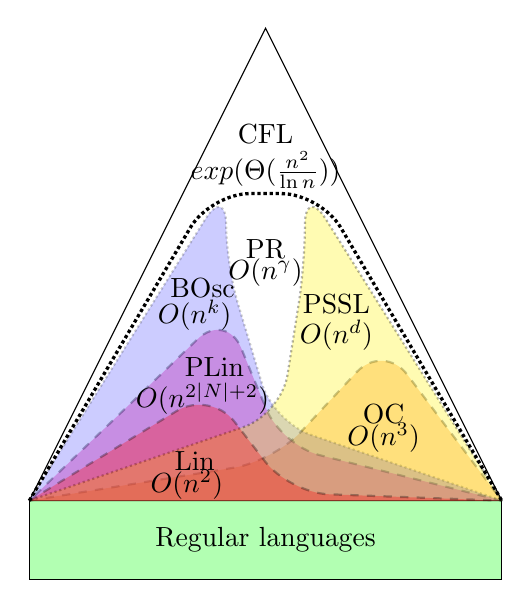
\begin{tikzpicture}
\draw[fill=green, opacity=0.3](0,1) -- (0,0) -- (6,0) --  (6,1);
\draw(0,1) -- (0,0) -- (6,0) --  (6,1);
\draw(0,1) -- (6,1) -- (3, 7) -- (0,1) ;
\draw[thick, dashed, rounded corners=5mm, fill=orange, opacity=0.3] (0,1) -- (3.1, 1.5) -- (4.5, 3) -- (6,1);
\draw[thick, dashed, rounded corners=5mm, fill=magenta, opacity=0.3] (6,1) -- (3.2, 1.7) -- (2.5, 3.4) -- (0,1);
\draw[thick, densely dotted, rounded corners=5mm, fill=blue, opacity=0.2](0,1) -- (2.5, 5) -- (2.5,4)-- (3.1, 2) -- (6,1);
\draw[thick, densely dotted, rounded corners=5mm , fill=yellow, opacity=0.3](6,1) -- (3.5, 5) -- (3.5,4)-- (3.2, 2.1) -- (0,1);
\draw[thick, dashed, rounded corners=5mm, fill=red, opacity=0.3] (0,1) -- (2.3, 2.4)  -- (3.3, 1.1) -- (6,1);
\draw[very thick, densely dotted, rounded corners=5mm] (0,1) -- (2.3, 4.9) -- (3.7, 4.9) -- (6,1);
\node (reg) at (3, 0.5) {Regular languages}; 
\node (cfl) at (3, 5.65) {CFL}; 
\node (pr) at (3, 4.2) {PR};
\node (prrho) at (3, 3.9) {$O(n^\gamma)$};
\node (cflrho) at (3, 5.2) {$exp(\Theta(\frac{n^2}{\ln n}))$}; 
\node (plin) at (2.35, 2.7) {PLin}; 
\node (lin) at (2.1, 1.5) {Lin}; 
\node (osc) at (2.2, 3.7) {BOsc}; 
\node (one) at (4.5, 1.8) {$O(n^3)$}; 
\node (onerho) at (4.5, 2.1) {OC}; 
\node (pssl) at (3.9,3.5) {PSSL}; 
\node (psslrho) at (3.9,3.1) {$O(n^{d})$}; 
\node (linrho) at (2, 1.2) {$O(n^2)$}; 
\node (linrho) at (2.2, 2.29) {$O(n^{2|N|+2})$}; 
\node (oscrho) at (2.1, 3.35) {$O(n^{k})$}; 
\end{tikzpicture}
\caption{The hierarchy of languages with polynomial rational indices and corresponding upper bounds on the value of rational index. PR --- the family of CFLs with a polynomial rational indices, BOsc --- bounded-oscillation languages, PSSL --- CFLs with poly-slender storage languages, PLin --- piecewise linear languages, OC --- one-counter languages, Lin --- linear languages, $n$ --- number of vertices in graph (NFA), $|N|$ --- the number of non-terminals of grammar in Chomsky normal form, $k$ --- the oscillation value, $d$ --- degree of polynomial density of a pushdown storage language, $\gamma$ --- algebraic number.}
\label{hierarchyfinal}      
\end{figure}
We have obtained two classes, which extend the classes in the recent literature \cite{ChainQ, labelledGraphs, LReach, Regularrealizability, Ullman}, for which CFL-reachability problem is in NC. The one is the class of bounded-oscillation languages, which generalizes the linear languages. The second class is context-free languages with a poly-slender pushdown store languages, which is generalization of the one-counter languages. Recall that regular languages have polynomial fringe property (and are accepted by PDA with a bounded stack height), also it is known that L-reachability for regular languages is in NL \cite{LReach, Yannakakis}. Thereby it has been demonstrated that some natural restrictions on the pushdown storage implies polynomial rational index for the corresponding context-free languages: low variability of stack height during the PDA run (bounded-oscillation PDA) and limited number of possible stack contents (languages with poly-slender pushdown store languages). The updated hierarchy of tractable subclasses and corresponding upper bounds on the rational indices are illustrated in Figure~\ref{hierarchyfinal}.


It will be interesting to know whether there is another kind of stack restriction which implies polynomial rational index. Or is there a context-free language which does not belong to any of the above mentioned classes? Are there any other properties (except polynomial rational index) which make the CFL-reachability problem solvable in NC? For example there is a Datalog query, which does not have a polynomial fringe property but its evaluation is in NC \cite{Kanellakis}. One can also approach this question from another direction by looking for simple subfamilies of context-free languages that would have P-complete CFL-reachability problem.


Also it is interesting to consider other machine models with stores having store restrictions examined in this work. Do these restrictions imply that certain properties can become decidable or decidable faster? Store languages of different machine models and their applications are studied in \cite{ Ibarra2018OnSL, IBARRA201928}.


We considered CFL-reachability problem for a fixed context-free languages and arbitrary graphs. What tractable cases can be obtained for a fixed graphs and an arbitrary context-free language? The known and trivial examples are acyclic graphs and trees. Can we have more complicated classes of graphs for which CFL-reachability problem is in NC? Interesting algebraic properties of such graphs (NFA) are given in \cite{ganardi2016circuit}, but automata-theoretic characterizations of these properties remain to be found.


%%For cite command type as \cite{1}; \cite{3,6} and \cite{2,4,6}.
%%For refcite command type as Refs.~[\refcite{1}];
%%[\refcite{1},\refcite{3}] and [\refcite{1}--\refcite{4}].


\section*{Acknowledgments}
This research was supported by the Russian Science Foundation, grant \textnumero 18-11-00100.



\bibliographystyle{ws-ijfcs}  
\bibliography{paper}
\end{document}